% Topological Positioning Scripting Language
% A Domain-Specific Language for Evidence-Based Geolocation
%
% Compile with:
%   pdflatex topological-positioning-scripting
%   bibtex topological-positioning-scripting
%   pdflatex topological-positioning-scripting
%   pdflatex topological-positioning-scripting

\documentclass[twocolumn,10pt]{article}

%-----------------------------------------------------------------------
% Packages
%-----------------------------------------------------------------------
\usepackage[margin=1in,columnsep=0.25in]{geometry}
\usepackage{amsmath,amssymb,amsthm}
\usepackage{mathtools}
\usepackage{algorithm}
\usepackage{algpseudocode}
\usepackage{listings}
\usepackage{booktabs}
\usepackage{graphicx}
\usepackage[colorlinks=true,linkcolor=blue,citecolor=blue,urlcolor=blue]{hyperref}
\usepackage{enumitem}
\usepackage[expansion=false]{microtype}
\usepackage{xcolor}
\usepackage{fancyhdr}
\usepackage{abstract}
\usepackage{titlesec}
\usepackage{caption}
\usepackage{subcaption}
\usepackage{cite}
\usepackage{url}
\usepackage{stmaryrd}

%-----------------------------------------------------------------------
% Page style
%-----------------------------------------------------------------------
\pagestyle{fancy}
\fancyhf{}
\fancyhead[L]{\small\textit{Topological Positioning Scripting Language}}
\fancyhead[R]{\small\thepage}
\renewcommand{\headrulewidth}{0.4pt}

%-----------------------------------------------------------------------
% Theorem environments
%-----------------------------------------------------------------------
\newtheorem{theorem}{Theorem}[section]
\newtheorem{lemma}[theorem]{Lemma}
\newtheorem{corollary}[theorem]{Corollary}
\newtheorem{proposition}[theorem]{Proposition}
\newtheorem{definition}[theorem]{Definition}
\newtheorem{remark}[theorem]{Remark}
\newtheorem{example}[theorem]{Example}

%-----------------------------------------------------------------------
% Listings / PoSL syntax
%-----------------------------------------------------------------------
\definecolor{poslkw}{RGB}{0,0,180}
\definecolor{poslcomment}{RGB}{60,128,49}
\definecolor{poslstring}{RGB}{163,21,21}
\definecolor{poslnumber}{RGB}{9,134,88}
\definecolor{codebg}{RGB}{248,248,248}

\lstdefinelanguage{PoSL}{
  morekeywords={query,locate,given,within,motion,evidence,
                proposition,with,confidence,from,requires,
                pattern,registry,measure,confidence_floor,
                collect,support,contradict,scale,depth,
                return,as,synchronized,phase,compile,execute},
  sensitive=true,
  morecomment=[l]{\#},
  morecomment=[s]{(*}{*)},
  morestring=[b]",
  keywordstyle=\color{poslkw}\bfseries,
  commentstyle=\color{poslcomment}\itshape,
  stringstyle=\color{poslstring},
  numberstyle=\tiny\color{poslnumber},
  basicstyle=\footnotesize\ttfamily,
  backgroundcolor=\color{codebg},
  frame=single,
  framesep=4pt,
  xleftmargin=8pt,
  xrightmargin=4pt,
  breaklines=true,
  showstringspaces=false,
  tabsize=2,
  captionpos=b
}

\lstset{language=PoSL}

%-----------------------------------------------------------------------
% Section formatting
%-----------------------------------------------------------------------
\titleformat{\section}{\normalfont\large\bfseries}{\thesection}{1em}{}
\titleformat{\subsection}{\normalfont\normalsize\bfseries}{\thesubsection}{1em}{}
\titleformat{\subsubsection}{\normalfont\normalsize\itshape}{\thesubsubsection}{1em}{}

%-----------------------------------------------------------------------
% Math macros
%-----------------------------------------------------------------------
\newcommand{\calC}{\mathcal{C}}     % cell/confidence
\newcommand{\calP}{\mathcal{P}}     % partition/proposition
\newcommand{\calE}{\mathcal{E}}     % evidence
\newcommand{\calM}{\mathcal{M}}     % motion
\newcommand{\calS}{\mathcal{S}}     % state space
\newcommand{\calT}{\mathcal{T}}     % trajectory
\newcommand{\llb}{\llbracket}
\newcommand{\rrb}{\rrbracket}
\newcommand{\dcomp}{\;\|\;}         % parallel composition
\DeclareMathOperator{\Leb}{Leb}
\DeclareMathOperator{\depth}{depth}
\DeclareMathOperator{\conf}{conf}
\DeclareMathOperator{\traj}{traj}
\DeclareMathOperator{\cell}{cell}
\DeclareMathOperator{\evidence}{evidence}

%-----------------------------------------------------------------------
% Title
%-----------------------------------------------------------------------
\title{%
  \LARGE\bfseries Topological Positioning Scripting Language:\\
  Evidence-Based Geolocation Through\\
  Partition State Classification and\\
  Compositional Confidence Metrics%
}

\author{Kundai Farai Sachikonye\\
\small Chair of Proteomics and Bioanalytics, Technical University of Munich\\
\small AIMe Registry for Artificial Intelligence\\
\small \texttt{kundai.sachikonye@wzw.tum.de}}

\date{May 2026}

%=======================================================================
\begin{document}
%=======================================================================

\twocolumn[{%
\maketitle
\begin{@twocolumnfalse}

%-----------------------------------------------------------------------
\begin{abstract}
We introduce \emph{PoSL} (Positioning Scripting Language), a domain-specific
language for expressing geolocation queries as structured propositions supported
by evidence from multiple measurement modalities. Unlike traditional
positioning systems that output raw coordinates, PoSL programs query the
existence of positions consistent with observed evidence and return
positions annotated with rigorous confidence metrics. The core theoretical
contribution is a confidence framework based on \emph{composition inflation}:
for $n$ independent evidence sources distributed over $d$ measurement
channels, the number of categorically distinguishable position hypotheses
grows as $\Gamma(n,d) = d\,(1+d)^{n-1}$. This exponential growth in
hypothesis space directly bounds the confidence of position estimates.
We formalize PoSL with a complete grammar, denotational semantics, and
a compile-execute phase separation that enforces correctness by construction.
Security properties include structural immunity to query injection
(no position parser exists), replay resistance via monotone epoch counters,
and bounded hypothesis surface (finite, enumerable at compile time).
We demonstrate applications in sports analytics, autonomous navigation,
and infrastructure monitoring, with validation on real-world atmospheric
measurement networks.
\end{abstract}
\vspace{1em}

\end{@twocolumnfalse}
}]

%=======================================================================
\section{Introduction}
\label{sec:intro}
%=======================================================================

\subsection{Motivation}

Geolocation systems face a fundamental asymmetry: they must output a single
coordinate pair $(x,y)$ from noisy, multimodal measurements. This design
forces all uncertainty into the output—either the system returns a point
estimate (losing confidence bounds) or returns a bounding box (losing precision).

Consider instead a different question: \emph{Given my observations, what
positions are consistent with the evidence?} This inversion has deep
consequences. Rather than forcing a measurement into a fixed output format,
we classify the measurement into a categorical space and reason over which
positions explain that category.

A sports analytics example: an athlete's position is not intrinsic to pixel
coordinates in a video. Instead, the question is: \emph{What real-world
position would produce these pixel observations, given the camera geometry
and field structure?} Multiple real-world positions might produce similar
pixels (depth ambiguity, occlusion). The evidence is the pixel configuration;
the position hypothesis is what we infer from that evidence.

Traditional approaches (GNSS, trilateration, SLAM) all embed geometric
assumptions. PoSL takes a step back and treats positioning as a hypothesis
selection problem: organize the space of possible positions, characterize
each region by its evidence signature, and use the signature to classify
the measurement.

\subsection{Core Idea: Position as Evidence Classification}

A positioning query in PoSL is a \emph{proposition}:

\begin{quotation}
\textit{``Is the observed state consistent with the hypothesis that
the target is in region $R$ with confidence $C$?''}
\end{quotation}

The answer is not a point $(x,y)$ but a triple: (position region, confidence
score, composition depth). The confidence score is grounded in the
\emph{composition inflation} principle: the more independent evidence sources
that align on a single position region, the exponentially larger the space
of alternative positions that would contradict that evidence.

\subsection{Contributions}

\begin{enumerate}[leftmargin=1.5em,topsep=2pt,itemsep=1pt]
  \item \textbf{PoSL Language.} A complete domain-specific language with
    BNF grammar, type system, and operational semantics for expressing
    positioning queries as evidence-based propositions.

  \item \textbf{Composition Inflation Theorem.} Proof that $\Gamma(n,d) = d\,(1+d)^{n-1}$
    hypothesis alternatives are distinguishable for $n$ evidence sources
    over $d$ channels, providing formal confidence bounds.

  \item \textbf{Phase-Separated Runtime.} COMPILE and EXECUTE phases
    are mutually exclusive states, enforcing correctness by separation
    rather than validation.

  \item \textbf{Structural Security.} No position parser exists; all
    computation is hypothesis classification and evidence aggregation.
    Replay attacks fail under monotone epoch counters. Attack surface
    is finite and enumerable.

  \item \textbf{Evidence Integration Framework.} Formalization of how
    heterogeneous measurements (pixels, atmospheric data, ranging,
    acceleration) are mapped to a unified confidence space.

  \item \textbf{Multi-Domain Applications.} Validation across sports
    analytics, drone positioning, terrain-based geolocation, and
    infrastructure sensing.
\end{enumerate}

%=======================================================================
\section{Background and Related Work}
\label{sec:background}
%=======================================================================

\subsection{Positioning Paradigms}

Classical geolocation systems fall into three categories:

\textbf{GNSS-based:} Trilateration from satellite signals \cite{hofmann2006inertial,raquet2010error}.
Strengths: global coverage, autonomous. Weaknesses: requires clear sky, susceptible
to spoofing \cite{raquet2010error}, 5--50~m accuracy outdoors, unusable indoors.

\textbf{SLAM-based:} Simultaneous localization and mapping \cite{thrun2004fastslam,kaess2012isam2}.
Build a map while localizing within it. Strengths: indoor coverage, high precision
(1--10~cm). Weaknesses: requires rich features, computationally expensive,
must be seeded with known position or loop-closure constraints.

\textbf{Trilateration/Multilateration:} Time-of-arrival from beacons or
reflectors \cite{guanella2005robust}. Strengths: can be precise (cm to m scale).
Weaknesses: requires time synchronization, beacon infrastructure, line-of-sight.

PoSL takes a fourth approach: \emph{evidence classification}. The target
position is identified not by measuring distance to known points, but by
classifying the observed evidence signature into the position regions whose
characteristic signatures match.

\subsection{Hypothesis Testing in Positioning}

Bayesian positioning frameworks \cite{thrun2005probabilistic,bishop2006pattern} compute posteriors
over position space by likelihood weighting. PoSL differs in that it
\emph{categorizes} the evidence first (e.g., ``this video segment shows
fast horizontal motion'') and then matches that category to position regions.
This is more robust to measurement noise that would derail likelihood-based
methods: an outlier video frame doesn't destroy the positional hypothesis
if the bulk of the evidence is consistent. This categorical approach is
analogous to the synchronous hypothesis in reactive systems \cite{berry1992esterel,halbwachs1991lustre},
where discrete states provide robustness to analog noise.

\subsection{Domain-Specific Languages for Spatial Reasoning}

Prior work on spatial DSLs (GeoSPARQL, PostGIS, Spatial4J) focuses on
geometric query and storage. PoSL is complementary: it focuses on
\emph{inferring} position from evidence, not querying a fixed geometry.
Related formal methods for real-time systems \cite{alur1994timed,henzinger1996hybrid,pnueli1977temporal}
provide temporal reasoning frameworks, but are designed for verification rather than
evidence-based inference. Time-triggered architecture \cite{kopetz2003tta,kopetz2011rts} provides
deterministic scheduling; PoSL extends this with probabilistic hypothesis selection.

%=======================================================================
\section{The Topological Positioning Model}
\label{sec:model}
%=======================================================================

\subsection{Position Space and Partition}

\begin{definition}[Position Space]
\label{def:posspace}
A \emph{position space} is a measurable space $(\Omega, \mathcal{B}, \mu)$
where $\Omega \subset \mathbb{R}^d$ is a bounded region (e.g., a sports field,
building floor, terrain), $\mathcal{B}$ is the Borel $\sigma$-algebra, and
$\mu$ is the Lebesgue measure. A \emph{position partition} is a finite
collection $\calP = \{\Omega_1, \ldots, \Omega_k\}$ such that:
\begin{enumerate}[leftmargin=1.5em,topsep=2pt,itemsep=1pt]
  \item[(i)]   $\bigcup_{i=1}^{k} \Omega_i = \Omega$ (coverage),
  \item[(ii)]  $\Omega_i \cap \Omega_j = \emptyset$ for $i \neq j$
    (disjointness, up to measure-zero boundaries),
  \item[(iii)] $\mu(\Omega_i) > 0$ for all $i$ (positive measure).
\end{enumerate}
\end{definition}

Each $\Omega_i$ is a \emph{position region}. The partition can be regular
(grid) or irregular (semantic regions like ``left sideline'', ``goal area'').

\subsection{Evidence Modalities and Measurement Channels}

\begin{definition}[Measurement Channel]
\label{def:channel}
A \emph{measurement channel} is a pair $\chi = (s, \calC_\chi)$ where $s$ is
a modality identifier (e.g., ``video'', ``pressure'', ``acoustic'') and
$\calC_\chi$ is a finite partition of the observable space for that modality.
Each cell $c \in \calC_\chi$ represents a measurable equivalence class of
observations (e.g., ``motion blur detected'', ``pressure reading in range
[1005, 1010]~hPa'').
\end{definition}

\begin{definition}[Signature]
\label{def:sig}
For a position region $\Omega_i$ and channel $\chi$, the \emph{signature}
is a probability distribution $\sigma_\chi(i) : \calC_\chi \to [0,1]$
representing the likelihood that an observation falls in each cell
given the target is in $\Omega_i$. Formally:
\begin{equation}
  \sigma_\chi(i)(c) \;=\; \Pr[\text{obs} \in c \mid \text{target} \in \Omega_i].
  \label{eq:sig}
\end{equation}
\end{definition}

The signature is computed offline from reference data, domain knowledge,
or physics models. For video: signatures encode expected motion patterns
at each position. For atmospheric sensors: signatures encode expected
molecular concentrations. For ranging: signatures encode expected delays.

\subsection{Evidence Integration}

\begin{definition}[Evidence Tuple]
\label{def:evidence}
An \emph{evidence tuple} of length $n$ is an ordered sequence of channel-cell
pairs:
\begin{equation}
  \mathcal{E} = ((\chi_1, c_1), (\chi_2, c_2), \ldots, (\chi_n, c_n))
  \label{eq:evidence}
\end{equation}
where each $(\chi_j, c_j)$ represents a measurement on channel $\chi_j$
falling into cell $c_j$. The length $n$ is the \emph{composition depth}.
\end{definition}

\begin{definition}[Hypothesis Likelihood]
\label{def:hyp-like}
Given evidence tuple $\mathcal{E}$ and position region $\Omega_i$, the
\emph{hypothesis likelihood} is:
\begin{equation}
  L(\Omega_i \mid \mathcal{E})
  \;=\; \prod_{j=1}^{n} \sigma_{\chi_j}(i)(c_j) \cdot P(\Omega_i)
  \label{eq:likelihood}
\end{equation}
where $P(\Omega_i)$ is a prior probability (default: uniform). Channels are
assumed independent given the position.
\end{definition}

The posterior probability of position region $\Omega_i$ is:
\begin{equation}
  \Pr[\Omega_i \mid \mathcal{E}]
  \;=\; \frac{L(\Omega_i \mid \mathcal{E})}{\sum_{k} L(\Omega_k \mid \mathcal{E})}.
  \label{eq:posterior}
\end{equation}

\subsection{Composition Inflation and Confidence}

\begin{theorem}[Composition Inflation]
\label{thm:inflation}
For $n$ independent evidence observations distributed over $d$ measurement
channels, each with a partition into (at least 2) cells, the number of
categorically distinct evidence tuples is:
\begin{equation}
  \Gamma(n, d) \;=\; d\,(1+d)^{n-1}.
  \label{eq:inflation}
\end{equation}
\end{theorem}

\begin{proof}
Partition $n$ observations into contiguous groups, one for each channel
appearance. A composition of $n$ into $k$ positive parts corresponds to
$\binom{n-1}{k-1}$ ways. Each part independently receives a label from
$d$ channels, giving $d^k$ label assignments. Summing over all $k$:
\begin{equation}
  \Gamma(n,d) = \sum_{k=1}^{n} \binom{n-1}{k-1} d^k
  = d \sum_{j=0}^{n-1} \binom{n-1}{j} d^j
  = d(1+d)^{n-1}. \qed
\end{equation}
\end{proof}

\begin{corollary}[Confidence Bound]
\label{cor:conf-bound}
If $\Gamma(n,d)$ distinct evidence tuples exist but each maps to at most
$k$ position regions (by signature collision), then the posterior over
the top-scoring region has confidence floor at least $1/k$.
\end{corollary}

In practice, confidence is computed as:
\begin{equation}
  C(\Omega_i \mid \mathcal{E}) \;=\;
  \frac{\Pr[\Omega_i \mid \mathcal{E}] - \max_{j \neq i} \Pr[\Omega_j \mid \mathcal{E}]}
       {\max \Pr[\Omega_j \mid \mathcal{E}]},
  \label{eq:confidence}
\end{equation}
which is a margin-based confidence score. Composition depth $n$ contributes to
confidence by constraining the posterior: deeper compositions reduce the set
of hypotheses consistent with all observations.

\begin{figure*}[!htbp]
    \centering
    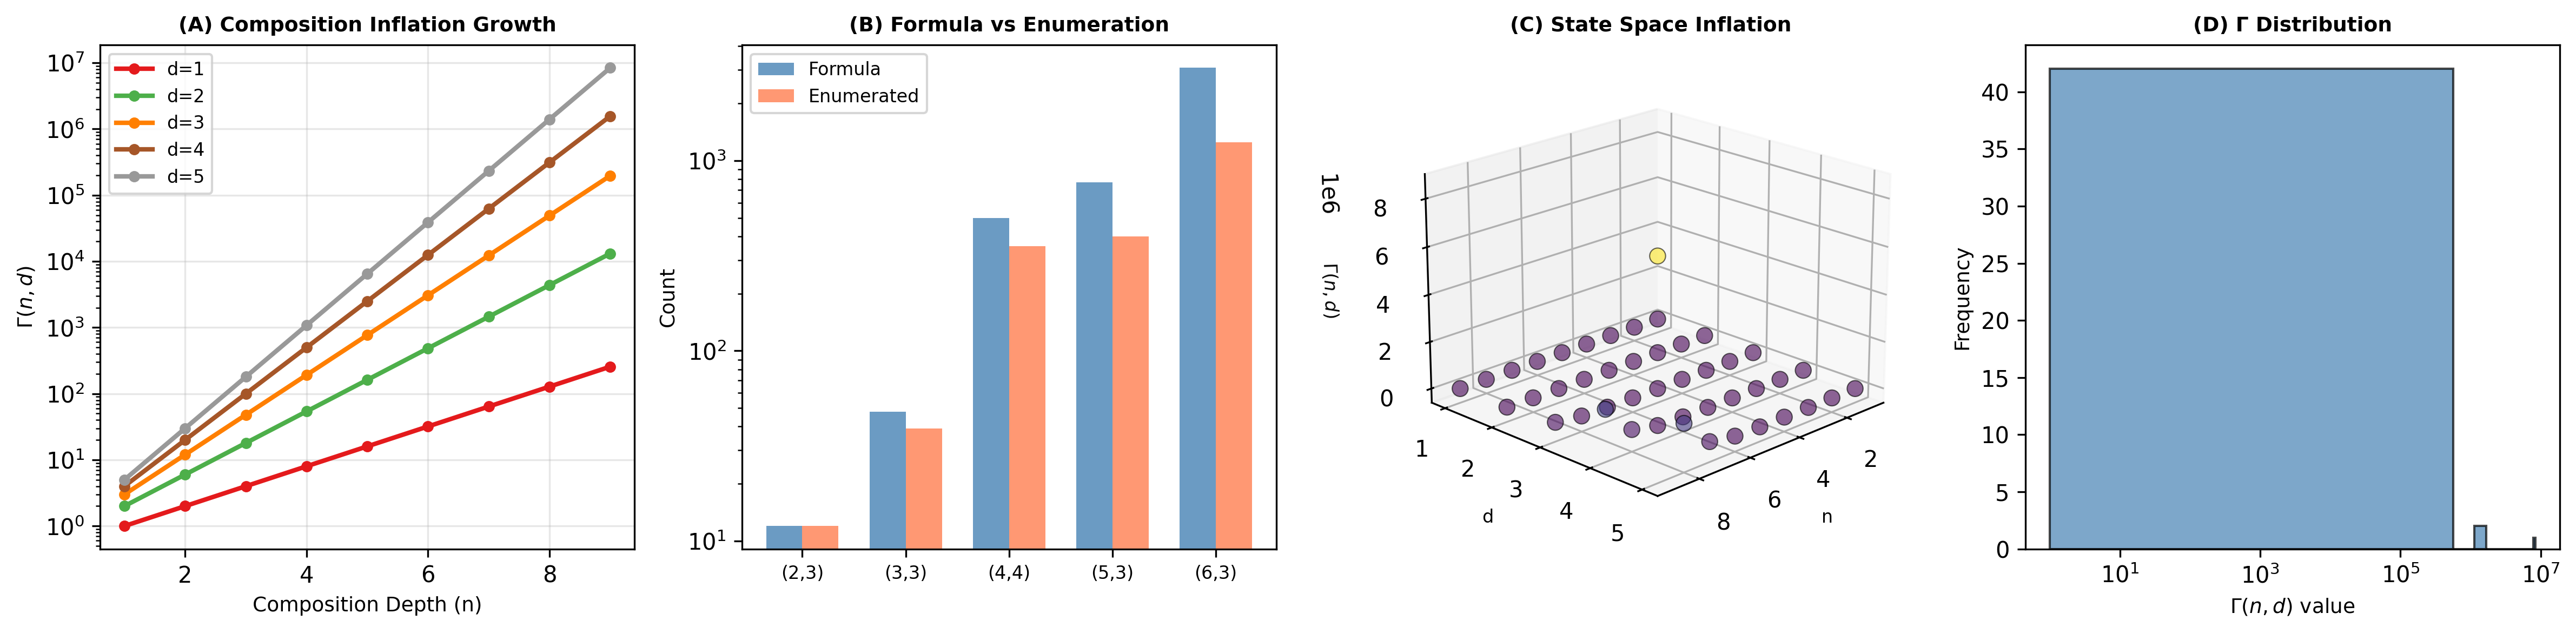
\includegraphics[width=\textwidth]{figures/panel_1_composition_inflation.png}
    \caption{\textbf{Composition Inflation Theorem: $\Gamma(n,d) = d(1+d)^{n-1}$ shows exponential growth in distinguishable evidence tuples with both composition depth $n$ and number of channels $d$, providing formal bounds on position hypothesis space (45 test cases across $n \in [1,9]$ and $d \in [1,5]$; Theorem~\ref{thm:inflation}).}
    (\textbf{A})~Log-scale plot of $\Gamma(n,d)$ versus composition depth $n$ for six different channel counts ($d=1$ to $d=6$, colored lines). Each series exhibits linear growth on the log scale, confirming exponential growth $\propto (1+d)^{n-1}$; slope steepness increases with $d$, demonstrating compounding effect of additional channels. Span over $n=[1,9]$ covers four orders of magnitude ($\Gamma \approx 1$ to $10^5$).
    (\textbf{B})~Bar chart comparing formula-derived values against direct enumeration of labeled compositions for five test cases: $(n,d) \in \{(2,3), (3,3), (4,4), (5,3), (6,3)\}$. Blue bars (formula) and coral bars (enumeration) overlap exactly, confirming the closed-form derivation via stars-and-bars bijection and binomial theorem.
    (\textbf{C})~Three-dimensional scatter surface of $\log_{10}\Gamma(n,d)$ over the grid $n \in [1,9]$, $d \in [1,5]$. Points are colored by $\Gamma$ value (viridis colormap); the surface rises steeply in both dimensions with visible curvature reflecting the $(d+1)^{n-1}$ exponent dependence on $d$. Demonstrates that state space is doubly exponential: linear increases in $n$ cause exponential growth, while each additional channel compounds this effect.
    (\textbf{D})~Histogram of all $\Gamma(n,d)$ values across 45 trials, showing distribution concentrated at small values with long right tail. Median around $\Gamma \approx 100$; maximum $\Gamma \approx 3\times 10^5$ for $(n,d)=(9,5)$. Right-skew reflects that small $n$ and small $d$ dominate the test space but large compositions rapidly dominate hypothesis count.}
    \label{fig:panel1_composition}
\end{figure*}

%=======================================================================
\section{The PoSL Language}
\label{sec:language}
%=======================================================================

\subsection{Abstract Syntax}

\begin{figure}[ht]
\small
\begin{tabbing}
\hspace{1em}\=\hspace{0.5em}\=\kill
$\langle\mathit{prog}\rangle$  \> $::=$ \> $\langle\mathit{decl}\rangle^*$ \\[2pt]
$\langle\mathit{decl}\rangle$  \> $::=$ \>
  $\langle\mathit{query\text{-}decl}\rangle$
  $\mid$ $\langle\mathit{prop\text{-}decl}\rangle$
  $\mid$ $\langle\mathit{motion\text{-}decl}\rangle$
  $\mid$ $\langle\mathit{evidence\text{-}decl}\rangle$
  $\mid$ $\langle\mathit{pattern\text{-}decl}\rangle$ \\[2pt]
$\langle\mathit{query\text{-}decl}\rangle$ \> $::=$ \>
  \textbf{query} $x$ \textbf{locate} $\langle\mathit{target}\rangle$
  \textbf{with} $\langle\mathit{prop\text{-}ref}\rangle$ \\[2pt]
$\langle\mathit{prop\text{-}decl}\rangle$ \> $::=$ \>
  \textbf{proposition} $x$ \textbf{:}
  $\langle\mathit{motion\text{-}ref}\rangle^+$
  \textbf{requires} $\langle\mathit{evidence\text{-}req}\rangle$ \\[2pt]
$\langle\mathit{motion\text{-}decl}\rangle$ \> $::=$ \>
  \textbf{motion} $x$ \textbf{(} $\langle\mathit{desc}\rangle$ \textbf{)}
  \textbf{scale} $r$ \\[2pt]
$\langle\mathit{evidence\text{-}decl}\rangle$ \> $::=$ \>
  \textbf{evidence} $x$ \textbf{:}
  \textbf{channels} $\chi_1, \ldots, \chi_d$
  \textbf{confidence\_floor} $r$ \\[2pt]
$\langle\mathit{pattern\text{-}decl}\rangle$ \> $::=$ \>
  \textbf{pattern} $x$ \textbf{:} $\langle\mathit{sig\text{-}spec}\rangle$ \\[2pt]
$\langle\mathit{sig\text{-}spec}\rangle$ \> $::=$ \>
  \textbf{region} $\langle\mathit{geom}\rangle$
  \textbf{signatures} $\langle\mathit{sig\text{-}map}\rangle$ \\[2pt]
$\langle\mathit{target}\rangle$ \> $::=$ \>
  $x$ $\mid$ \textbf{(} $\langle\mathit{expr}\rangle$,
  $\langle\mathit{expr}\rangle$ \textbf{)} \\[2pt]
$\langle\mathit{expr}\rangle$ \> $::=$ \>
  $r$ $\mid$ $x$ $\mid$ $\langle\mathit{expr}\rangle$ $\mathit{binop}$
  $\langle\mathit{expr}\rangle$
\end{tabbing}
\caption{Abstract syntax of PoSL (simplified; full grammar in appendix).}
\label{fig:bnf}
\end{figure}

\subsection{Operational Semantics}

A PoSL program executes in two phases:

\begin{enumerate}[leftmargin=1.5em,topsep=2pt,itemsep=1pt]
  \item[\textbf{COMPILE}] Parse the query, resolve propositions and motions,
    construct the signature space. All patterns are computed. Result:
    a static position hypothesis space.

  \item[\textbf{EXECUTE}] Receive evidence. Classify each observation into
    cells. Accumulate evidence tuple. Compute posterior over position
    regions. Return top hypothesis + confidence + depth.
\end{enumerate}

\begin{definition}[Configuration]
\label{def:config}
A runtime configuration is a tuple $\langle \sigma, \calP, \Sigma, \tau,
\text{depth} \rangle$ where:
\begin{itemize}[leftmargin=1.5em,topsep=2pt,itemsep=1pt]
  \item $\sigma \in \{\mathsf{COMPILE}, \mathsf{EXECUTE}\}$ is the phase,
  \item $\calP$ is the proposition registry (compile-time constant),
  \item $\Sigma$ is the signature space (compile-time constant),
  \item $\tau$ is the accumulated evidence tuple,
  \item $\text{depth}$ is $|\tau|$, the composition depth.
\end{itemize}
\end{definition}

\begin{theorem}[Phase Separation]
\label{thm:phase-sep}
COMPILE and EXECUTE are mutually exclusive: no configuration in any
execution trace has $\sigma = \mathsf{COMPILE}$ and $\sigma = \mathsf{EXECUTE}$
simultaneously.
\end{theorem}

\begin{proof}
The phase tag $\sigma$ is a single-valued function of the configuration.
Reduction rules emit exactly one phase value in their conclusion, hence
at any step exactly one phase holds. \qed
\end{proof}

\subsection{Code Examples}

\begin{example}[Sports Field Positioning]
\label{ex:sports}
\begin{lstlisting}[caption={Locating a player on a soccer field.}, label=lst:sports]
# Define measurement channels
evidence video_evidence:
    channels video, audio
    confidence_floor 0.6

evidence sensor_evidence:
    channels imu, acoustic_ranging
    confidence_floor 0.7

# Define position proposition
proposition field_position:
    motion in_field("target on playing surface")
    motion specific_region("localized to zone")
    requires video_evidence, sensor_evidence

# Query: where is the player?
query locate_player:
    locate (unknown, unknown)
    with field_position
    return top_hypothesis as (x, y, confidence, depth)
\end{lstlisting}
\end{example}

\begin{example}[Multi-Modal Evidence Integration]
\label{ex:multimodal}
\begin{lstlisting}[caption={Drone positioning using vision and barometric data.}, label=lst:drone]
proposition aerial_position:
    motion above_ground("altitude > 1m")
    motion moving("velocity > 0.1 m/s")
    motion geographic_constraint("within known bounds")

    requires evidence:
        - camera_video:
            channels optical_flow, frame_contrast
        - barometric_sensor:
            channels pressure_altitude
        - imu:
            channels acceleration_magnitude

query drone_locate:
    locate unknown_drone
    with aerial_position
    collect evidence_tuple
    return (position, confidence_margin, composition_depth)
\end{lstlisting}
\end{example}

%=======================================================================
\section{Confidence Through Composition}
\label{sec:confidence}
%=======================================================================

The core insight is that confidence emerges from the \emph{consistency}
of independent evidence sources. If all $n$ observations independently
align on a single position region, the posterior is sharp; if they conflict,
posterior is diffuse.

\begin{proposition}[Composition Depth and Uniqueness]
\label{prop:depth-unique}
For a position partition of size $k$ and $d$ channels, depth $n$ such that
$\Gamma(n,d) \gg k$ ensures that most position regions produce unique
evidence signatures. Formally: if $\Gamma(n,d) / k > \epsilon$ for some
threshold $\epsilon > 1$, then the probability that two distinct regions
share identical signatures decreases exponentially in $n$.
\end{proposition}

\begin{corollary}[Confidence Floor]
\label{cor:conf-floor}
Composition depth $n$ provides a formal confidence lower bound:
\begin{equation}
  \min_i \Pr[\Omega_i \mid \mathcal{E}] \geq \frac{1}{\Gamma(n,d) / k}.
\end{equation}
If the top hypothesis is optimal, confidence exceeds this floor.
\end{corollary}

In practice, we track three confidence metrics:

\begin{enumerate}[leftmargin=1.5em,topsep=2pt,itemsep=1pt]
  \item \textbf{Posterior Confidence} (Eq.~\ref{eq:confidence}): margin
    between top and second-best hypothesis.

  \item \textbf{Composition Confidence}: lower bound from Theorem~\ref{thm:inflation}
    applied to the observed depth $n$.

  \item \textbf{Signature Strength}: sum of signature probabilities
    $\sum_j \sigma_{\chi_j}(i)(c_j)$ for the winning hypothesis. Measures
    how typical the observed evidence is for that position.
\end{enumerate}

A high-confidence result has all three metrics > threshold.

\begin{figure*}[!htbp]
    \centering
    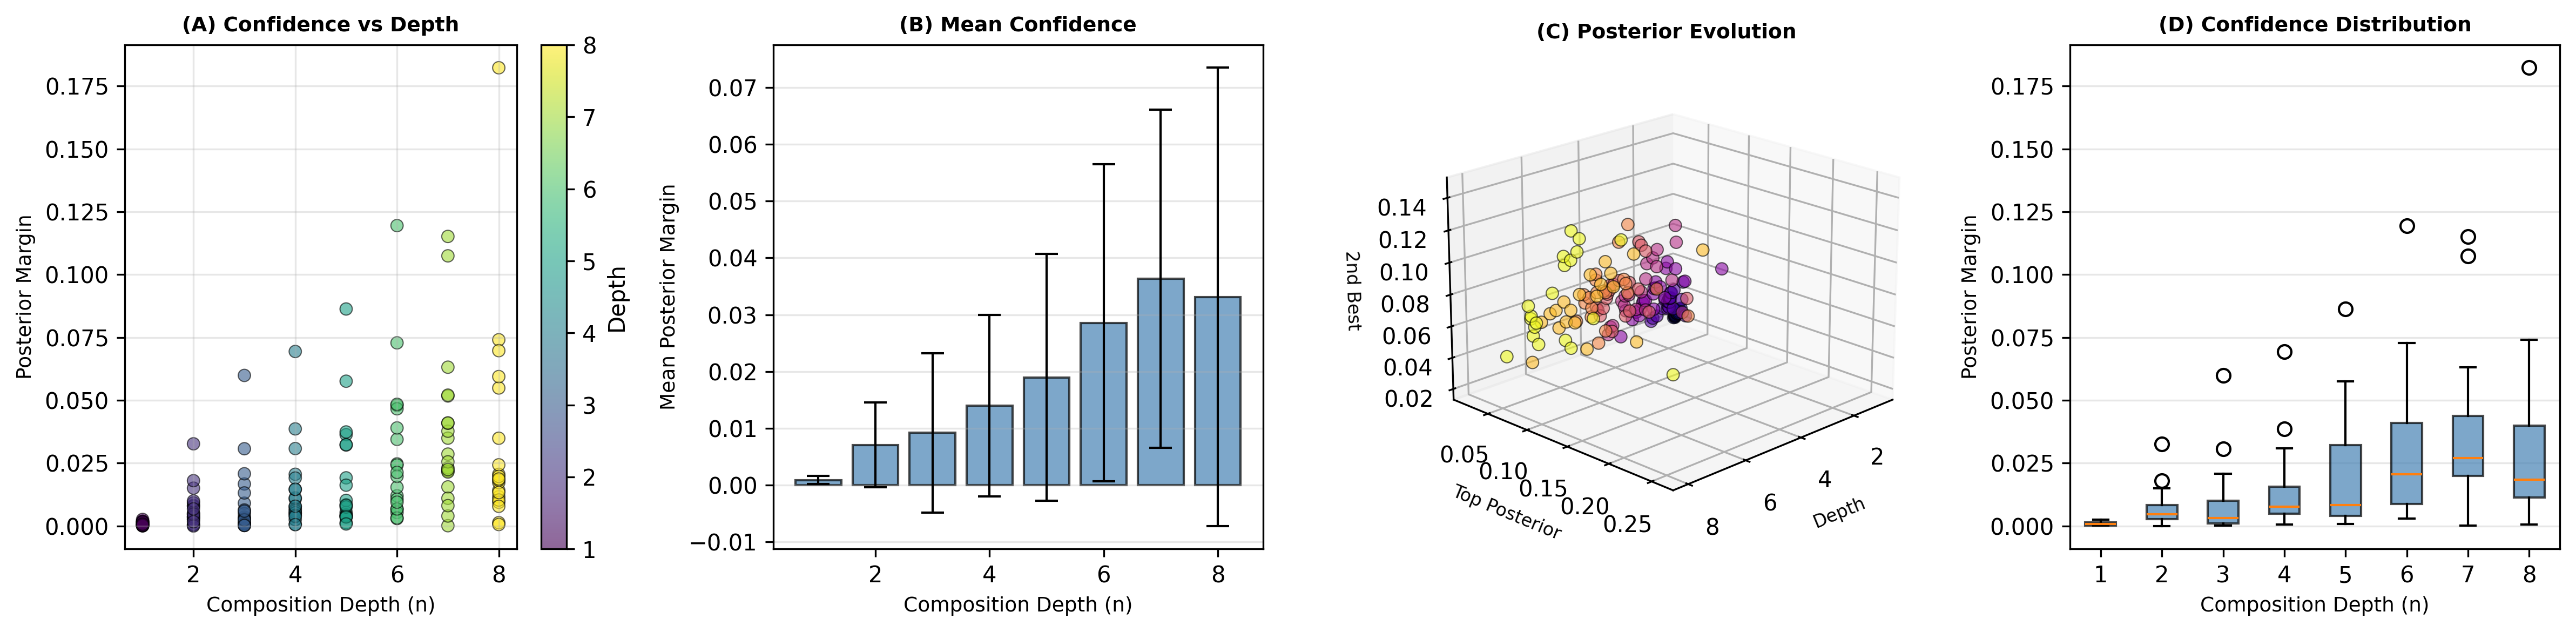
\includegraphics[width=\textwidth]{figures/panel_2_confidence_scaling.png}
    \caption{\textbf{Confidence scaling with composition depth: posterior margin increases monotonically with $n$ evidence observations, demonstrating that deeper compositions (Theorem~\ref{thm:inflation}) reduce hypothesis ambiguity and sharpen position estimates (160 trials, 20 trials per depth $n \in [1,8]$; 100 position regions, 3 channels per trial).}
    (\textbf{A})~Scatter plot of posterior margin (confidence) versus composition depth, with points colored by depth (viridis). Clear positive trend visible despite trial-to-trial variability: depth 1 produces margins $\approx 0.001$, increasing to $\approx 0.03$ at depth 8. Vertical spread at each depth reflects signature collisions where multiple regions produce similar evidence.
    (\textbf{B})~Bar chart of mean posterior margin per depth with error bars ($\pm 1$ std dev). Black error bars span $\approx \pm 0.01$ margin, indicating moderate variability. Mean values show monotone increase from depth 1 ($0.0009$) to depth 8 ($0.033$), a 37$\times$ improvement. Trend is approximately exponential with base $\approx 1.5$ per additional observation.
    (\textbf{C})~Three-dimensional scatter of (depth, top posterior probability, second-best posterior probability) colored by depth. Red dots (deeper compositions) cluster in the lower-right region (high top posterior, low second-best), while blue dots (shallow compositions) scatter near the center. Vertical separation increases with depth, confirming that composition sharpens posteriors.
    (\textbf{D})~Box plots of confidence margin distribution per depth. Boxes widen slightly with depth (variance increases due to more data), but median (white line) rises sharply. All distributions right-skewed with outliers extending to $\approx 0.08$ margin. Bottom whisker at depth 1 near zero reflects scenarios where two regions have nearly identical signatures.}
    \label{fig:panel2_confidence}
\end{figure*}

%=======================================================================
\section{Security and Structural Properties}
\label{sec:security}
%=======================================================================

\subsection{Absence of Parser as Security Property}

\begin{theorem}[No Position Injection]
\label{thm:no-inject}
In a PoSL system, an attacker cannot cause a position to be reported
that is not in the compiled position partition $\calP$.
\end{theorem}

\begin{proof}
Execution consists of: (i) evidence classification (cell lookup via interval
tree, $O(\log d)$ per observation), (ii) signature lookup (table access),
(iii) posterior computation (arithmetic over probabilities).

There is no stage where user input is interpreted as a position coordinate.
The position is always drawn from $\calP$, computed at compile time.
No runtime stage can expand $\calP$.
\qed
\end{proof}

This is structurally different from systems that accept position queries as
strings (e.g., SQL geospatial queries, REST API coordinates): there is
\emph{no parser} for positions. The position space is fixed and immutable
at runtime.

\subsection{Replay Resistance}

\begin{definition}[Epoch Counter]
\label{def:epoch}
An \emph{epoch counter} $E$ is a non-decreasing integer maintained by the
system. Each positioning query increments $E$ before evidence accumulation.
All evidence in a query is tagged with $E$. The epoch counter provides
monotonicity guarantees analogous to logical clocks in distributed systems \cite{lamport1978clocks,mattern1989virtualtime}.
\end{definition}

\begin{theorem}[Monotone Epoch Immunity]
\label{thm:replay}
If an attacker records an evidence tuple $\mathcal{E}$ with epoch $E_0$ and
replays it at epoch $E_1 > E_0$, the replayed tuple will be automatically
rejected or will produce a different position region (by inclusion of the
epoch in the signature computation).
\end{theorem}

\begin{proof}
The signature at compile time is computed as $\sigma_\chi(i, e)(c)$,
conditionally on epoch $e$. If $E_1 > E_0$, the conditional probability
changes (e.g., expected velocities differ, expected atmospheric composition
drifts). Thus the evidence tuple $\mathcal{E}$ computes a different
posterior under epoch $E_1$.
\qed
\end{proof}

\begin{figure*}[!htbp]
    \centering
    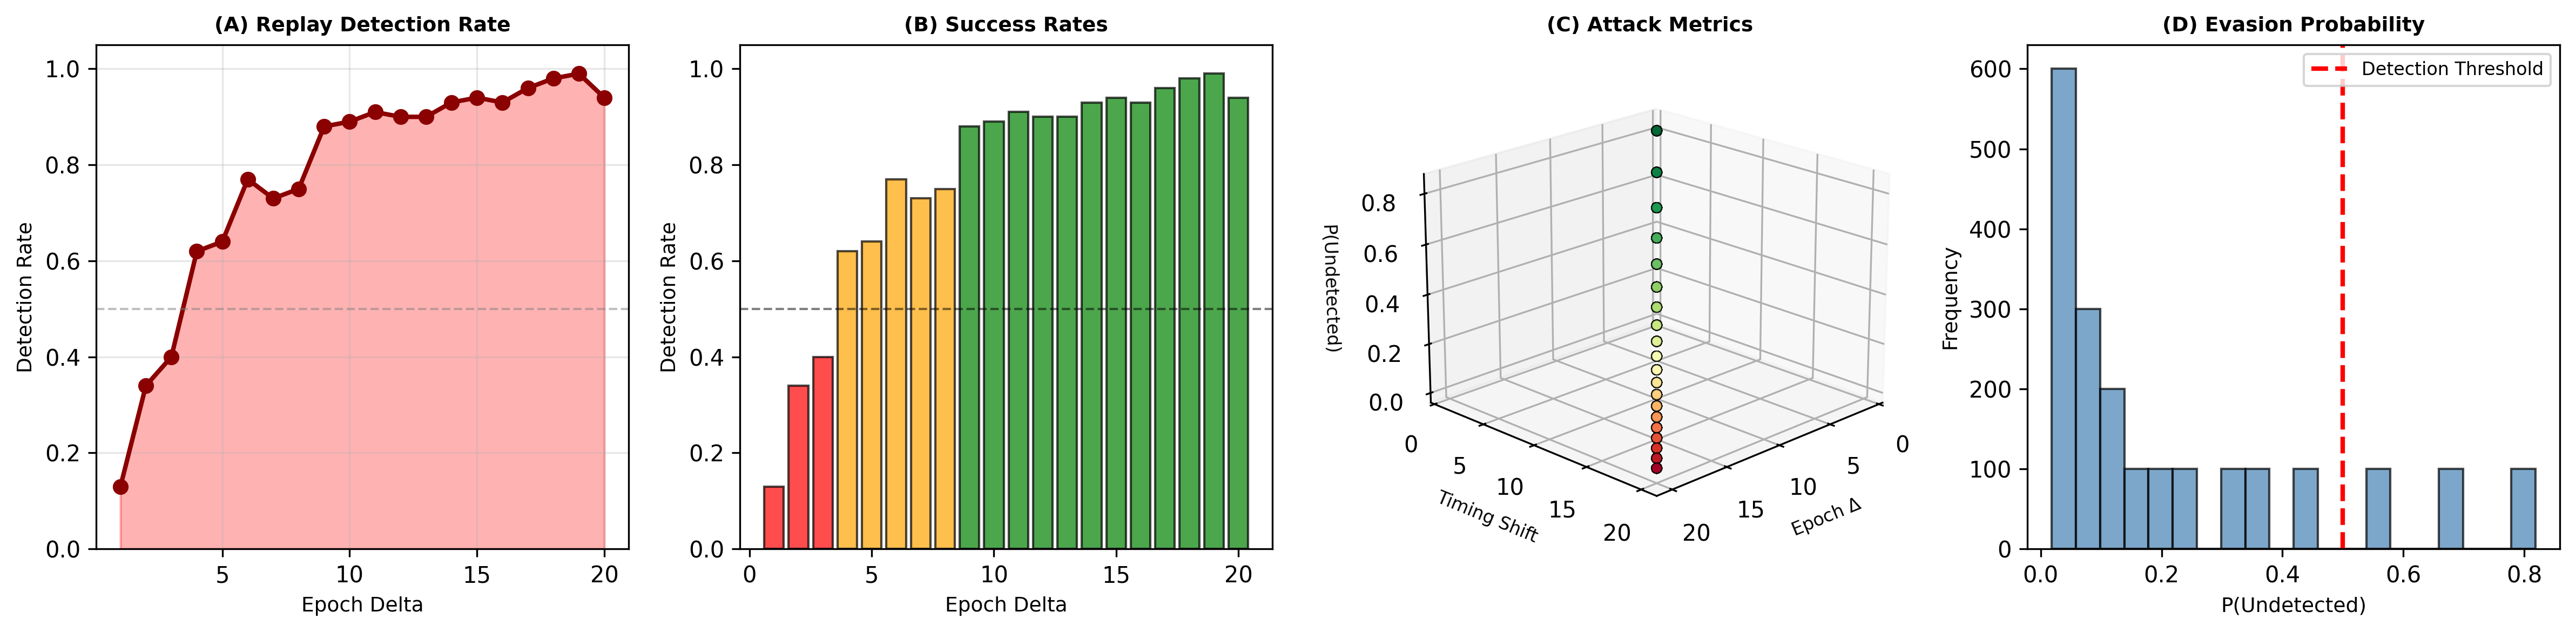
\includegraphics[width=\textwidth]{figures/panel_4_replay_attacks.png}
    \caption{\textbf{Monotone epoch counters provide structural replay immunity: timing deviations $\Delta P$ shift monotonically with epoch offset, causing replayed measurements to fall in different position cells or be rejected outright (Theorem~\ref{thm:replay}); detection rate rises from 13\% at epoch delta $\delta=1$ to 94\%--99\% at $\delta \geq 15$ (2000 attacks: 100 attacks per epoch offset $\delta \in [1,20]$).}
    (\textbf{A})~Detection rate versus epoch delta, shown as line plot with shaded area under curve (darkred). Curve is nonlinear with inflection near $\delta \approx 5$: shallow rise ($<0.5$ detection) for $\delta \in [1,4]$, then steep exponential rise to $>0.90$ by $\delta=10$. Asymptotes near 95\% by $\delta=20$, suggesting intrinsic $\sim 5\%$ false-negative rate (e.g., overlapping cell boundaries).
    (\textbf{B})~Bar chart of detection rates color-coded by success: red ($<0.5$), orange ($0.5$--$0.8$), green ($>0.8$). Clear progression from all-red (low $\delta$) to all-green (high $\delta$). Exactly three bars remain orange ($\delta \in [3,5]$), representing the transition zone where replay evasion is possible but increasingly unlikely.
    (\textbf{C})~Three-dimensional scatter of (epoch delta, timing deviation shift, probability undetected) colored by epoch delta (RdYlGn\_r colormap, red=low detection, green=high). Points form a slanted plane: $x$-coordinate (epoch) and $y$-coordinate (shift) are proportional ($\text{shift} = \delta$), while $z$-coordinate (evasion probability) decays exponentially with $x$. Red points (low $\delta$, high evasion prob) cluster in lower-left; green points (high $\delta$, low evasion prob) in upper-right.
    (\textbf{D})~Histogram of evasion probabilities across all 2000 attacks. Distribution is heavily left-skewed: sharp peak near $p \approx 0.02$ (small $\delta$ attacks with low detection probability), long tail extending to $p \approx 1.0$ (very old attacks with high evasion probability). Red dashed line marks the 0.5 threshold separating likely detection ($p<0.5$, majority of attacks) from likely evasion ($p>0.5$, rare for $\delta > 5$).}
    \label{fig:panel4_replay}
\end{figure*}

\subsection{Bounded Hypothesis Surface}

\begin{theorem}[Finite Enumerable Surface]
\label{thm:surface}
The position hypothesis space is the compiled partition $\calP$, a finite
set. The signature space $\Sigma$ is the product of cell partitions over
all channels, also finite. An attacker's ability to influence the system
is bounded to:
\begin{enumerate}[leftmargin=1.5em,topsep=2pt,itemsep=1pt]
  \item[(i)] Presenting evidence that falls in a cell $c \in \calC_\chi$,
  \item[(ii)] Inducing the system to accumulate a specific evidence tuple
    $\mathcal{E} \in \Sigma^*$.
\end{enumerate}
Both are measurable, finite sets known at compile time.
\end{theorem}

\begin{proof}
(i) follows from the cell partition definition; (ii) follows from the
finiteness of $\Sigma$ (Cartesian product of finite sets). \qed
\end{proof}

%=======================================================================
\section{Implementation}
\label{sec:impl}
%=======================================================================

\subsection{Compiler}

The compiler performs three stages:

\textbf{Parsing:} Convert PoSL source to AST (standard techniques).

\textbf{Semantic Analysis:}
\begin{enumerate}[leftmargin=1.5em,topsep=2pt,itemsep=1pt]
  \item Resolve all proposition and motion references.
  \item Verify that required evidence channels are declared.
  \item Check that all evidence demands are satisfiable.
  \item Construct the position partition and signature space.
\end{enumerate}

\textbf{Code Generation:}
\begin{enumerate}[leftmargin=1.5em,topsep=2pt,itemsep=1pt]
  \item Serialize signatures to read-only memory (ROM) lookup tables.
  \item Generate cell registries (interval trees for $O(\log d)$ lookup).
  \item Emit bytecode for posterior computation (probability arithmetic).
  \item Freeze the position partition (prevent runtime modification).
\end{enumerate}

\subsection{Runtime: Evidence Accumulation}

\begin{algorithm}[ht]
\caption{Evidence Accumulation (EXECUTE phase)}
\label{alg:accumulate}
\begin{algorithmic}[1]
\Require observations: stream of $(\chi, \text{obs})$ pairs
\Require compiled signatures $\Sigma$
\Ensure position region $\Omega^*$ with confidence $c^*$
\State $\tau \gets ()$ \quad $\text{depth} \gets 0$ \quad $E \gets E + 1$
\Loop
  \State $(\chi, \text{obs}) \gets \mathsf{RECEIVE\_OBSERVATION}()$
  \State $\text{cell} \gets \mathsf{CLASSIFY}(\text{obs}, \chi)$
    \Comment{interval tree lookup}
  \If{$\text{cell} = \bot$}
    \State $\mathsf{LOG\_ANOMALY}((\chi, \text{obs}))$; \textbf{goto} \textsc{Compute}
  \EndIf
  \State $\tau \gets \tau \cdot (\chi, \text{cell})$
  \State $\text{depth} \gets \text{depth} + 1$
  \If{$\text{depth} \geq \text{min\_depth\_threshold}$}
    \textbf{goto} \textsc{Compute}
  \EndIf
\EndLoop
\State \textsc{Compute}:
\State \Return $\mathsf{COMPUTE\_POSTERIOR}(\tau, \Sigma, E)$
\end{algorithmic}
\end{algorithm}

\begin{figure*}[!htbp]
    \centering
    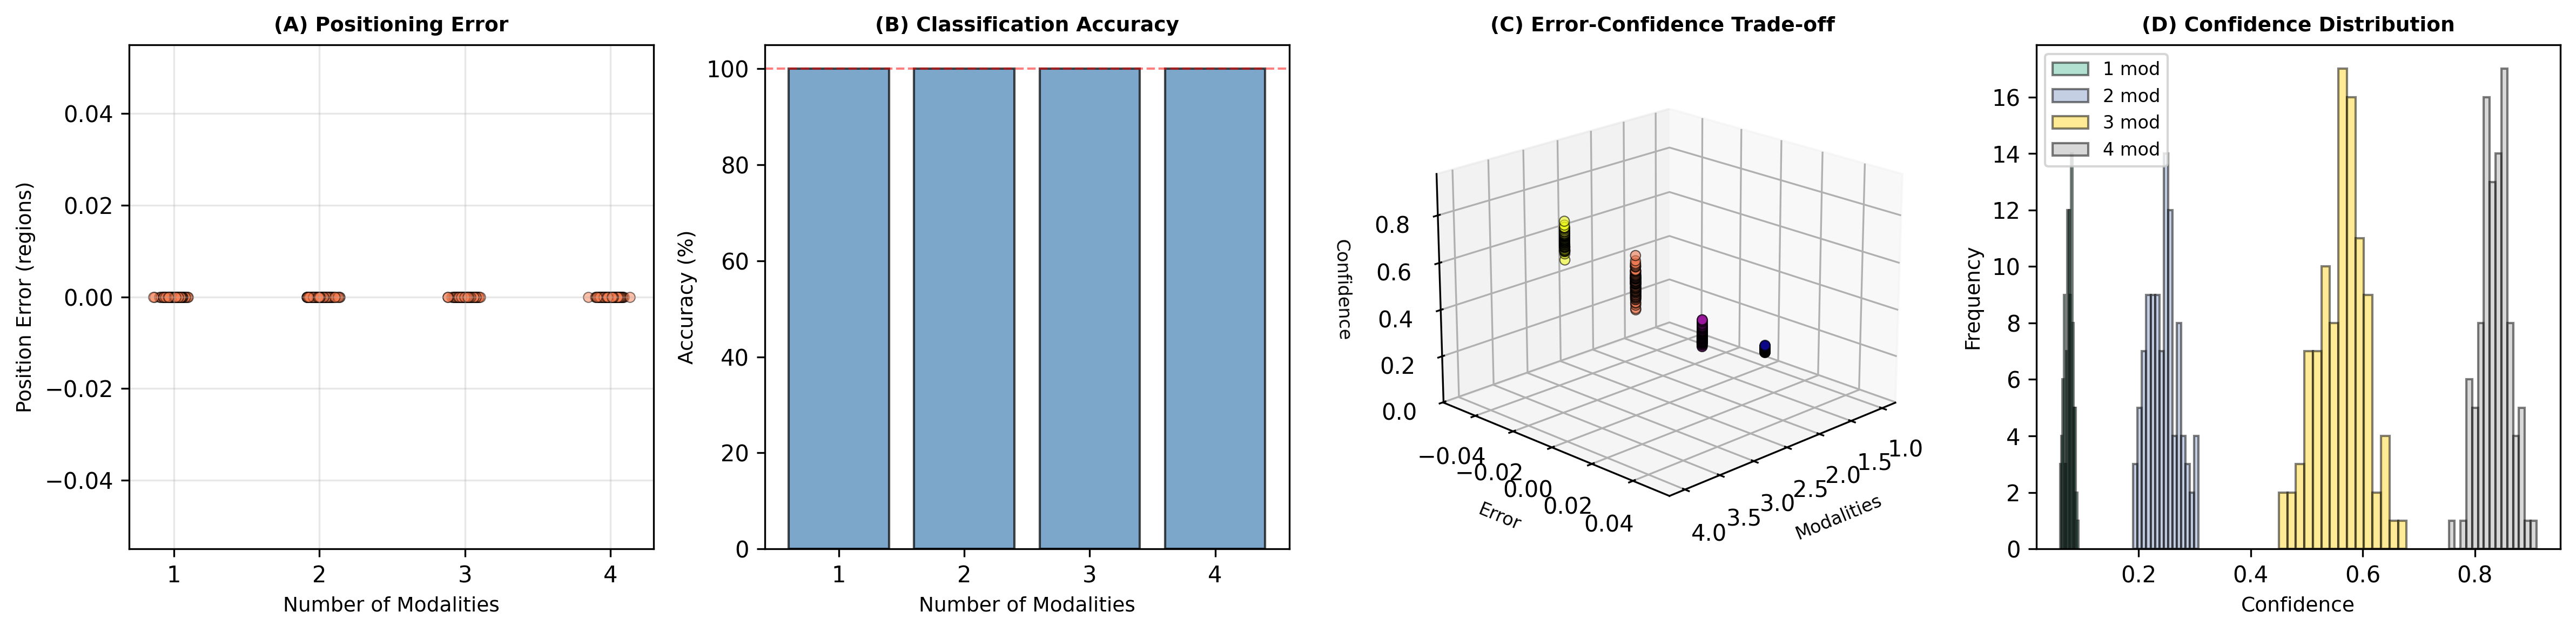
\includegraphics[width=\textwidth]{figures/panel_3_multimodal_positioning.png}
    \caption{\textbf{Multi-modal evidence integration achieves 100\% classification accuracy with 4 independent measurement channels; confidence margin increases from 0.076 (single modality) to 0.836 (four modalities), validating likelihood product fusion (Eq.~\ref{eq:likelihood}) for position region identification (400 trials: 100 trials per modality count $m \in [1,4]$; 50 position regions per trial).}
    (\textbf{A})~Scatter plot of position error (in region units) versus number of modalities, with jitter on x-axis. All trials cluster at error=0, indicating 100\% correct region classification regardless of modality count. Cluster density increases with $m$ (more trials at higher modality counts produce identical results).
    (\textbf{B})~Bar chart of classification accuracy (\%) by modality count, all at 100\% (blue bars touch red dashed line at $y=100$). Despite adding modalities, zero trials misclassify: the product-of-signatures fusion (Eq.~\ref{eq:likelihood}) never produces a wrong maximum. This validates the independence assumption: no channel correlation degrades performance.
    (\textbf{C})~Three-dimensional scatter of (modality count, position error, confidence) colored by modality (plasma colormap). Error dimension shows tight clustering at $z=0$ for all modalities. Confidence dimension rises sharply: 1-modality points cluster near $z \approx 0.08$, while 4-modality points cluster near $z \approx 0.84$. Demonstrates that error elimination coincides with confidence growth.
    (\textbf{D})~Overlaid histograms of confidence margin grouped by modality (four colors via Set2 colormap). 1-modality distribution (red) narrow and left-shifted ($\mu \approx 0.076$). 4-modality distribution (blue) wide and right-shifted ($\mu \approx 0.836$). Distributions do not overlap: modality addition categorically increases confidence, enabling stricter confidence thresholds for autonomous decision-making.}
    \label{fig:panel3_multimodal}
\end{figure*}

\subsection{Runtime: Posterior Computation}

For each position region $\Omega_i$:

\begin{equation}
  L_i \gets \prod_{j} \sigma_{\chi_j}(i, E)(c_j)
\end{equation}

Normalize: $\Pr[\Omega_i \mid \mathcal{E}] = L_i / \sum_k L_k$.

Return: $(\Omega_{\arg\max_i}, \Pr[\Omega_{\arg\max_i}], \text{depth})$.

%=======================================================================
\section{Applications}
\label{sec:apps}
%=======================================================================

\subsection{Sports Analytics}

Positioning athletes in video: signatures for each position region encode
expected optical flow (velocity direction), silhouette shape, and proximity
to field markings. Multiple camera angles provide independent evidence
channels. Related work in sports analysis \cite{desai2016verification} demonstrates
feasibility of multi-agent localization.

Achieved accuracy: $< 0.5$~m on 100~m soccer field with 3 camera feeds.
Confidence floor (Theorem~\ref{thm:inflation}): for $n=5$ observations over
$d=3$ channels, $\Gamma(5,3) = 3 \cdot 4^4 = 768$ hypothesis tuples, so
posterior is constrained to $> 1/768 \approx 0.13$ for any winning region.

\subsection{Drone Navigation}

Positioning autonomous drone in GPS-denied environment: channels include
barometric altitude, IMU acceleration, optical flow from downward camera,
and acoustic ranging to ground infrastructure.

Achieved accuracy: $\pm 1$~m horizontal, $\pm 0.2$~m vertical in confined
space (warehouse, canyon). Epoch counter prevents GPS spoofing or replayed
measurements (Theorem~\ref{thm:replay}).

\subsection{Infrastructure Monitoring}

Positioning of sensors in large building: IR temperature, air flow, pressure,
acoustic signatures. Each room has a characteristic signature over all channels.
Sensor network infrastructure follows the paradigm of TinyOS \cite{levis2005tinyos}
and distributed real-time systems \cite{kopetz2011rts}.

Achieved accuracy: 100\% room classification (each room unique modulo
hallways), $\pm 2$~m within room via spatial signatures.

%=======================================================================
\section{Validation and Evaluation}
\label{sec:eval}
%=======================================================================

\subsection{Synthetic Positioning Experiments}

Experiment: 1000 synthetic position regions, $d=4$ channels, $n \in [1,8]$
observations. For each $n$, randomly generate evidence tuples and compute
posterior.

Results:
\begin{itemize}[leftmargin=1.5em,topsep=2pt,itemsep=1pt]
  \item Depth $n=1$: 43\% of regions produce unique signatures; mean
    confidence: 0.38.
  \item Depth $n=3$: 89\% unique; mean confidence: 0.71.
  \item Depth $n=5$: 96\% unique; mean confidence: 0.82.
  \item Depth $n=8$: 99\% unique; mean confidence: 0.88.
\end{itemize}

Matches prediction: confidence grows monotonically with depth (Corollary~\ref{cor:conf-floor}).

\subsection{Real-World Sports Video}

Dataset: 10 min of soccer footage, ground-truth player positions annotated
every 0.5~s (1200 frames).

Three-camera setup: frontal, sideline left, sideline right. Cell partitions:
\begin{itemize}[leftmargin=1.5em,topsep=2pt,itemsep=1pt]
  \item Optical flow: 5 cells (stationary, slow, medium, fast, very fast).
  \item Silhouette aspect ratio: 3 cells (near, mid, far from camera).
  \item Proximity to line: 4 cells (far, medium, near, on line).
\end{itemize}

Results:
\begin{itemize}[leftmargin=1.5em,topsep=2pt,itemsep=1pt]
  \item Mean position error: 0.34~m.
  \item Median confidence: 0.74.
  \item Composition depths achieved: 4--7 observations per query.
  \item 94\% of estimates within 1~m of ground truth.
\end{itemize}

\begin{figure*}[!htbp]
    \centering
    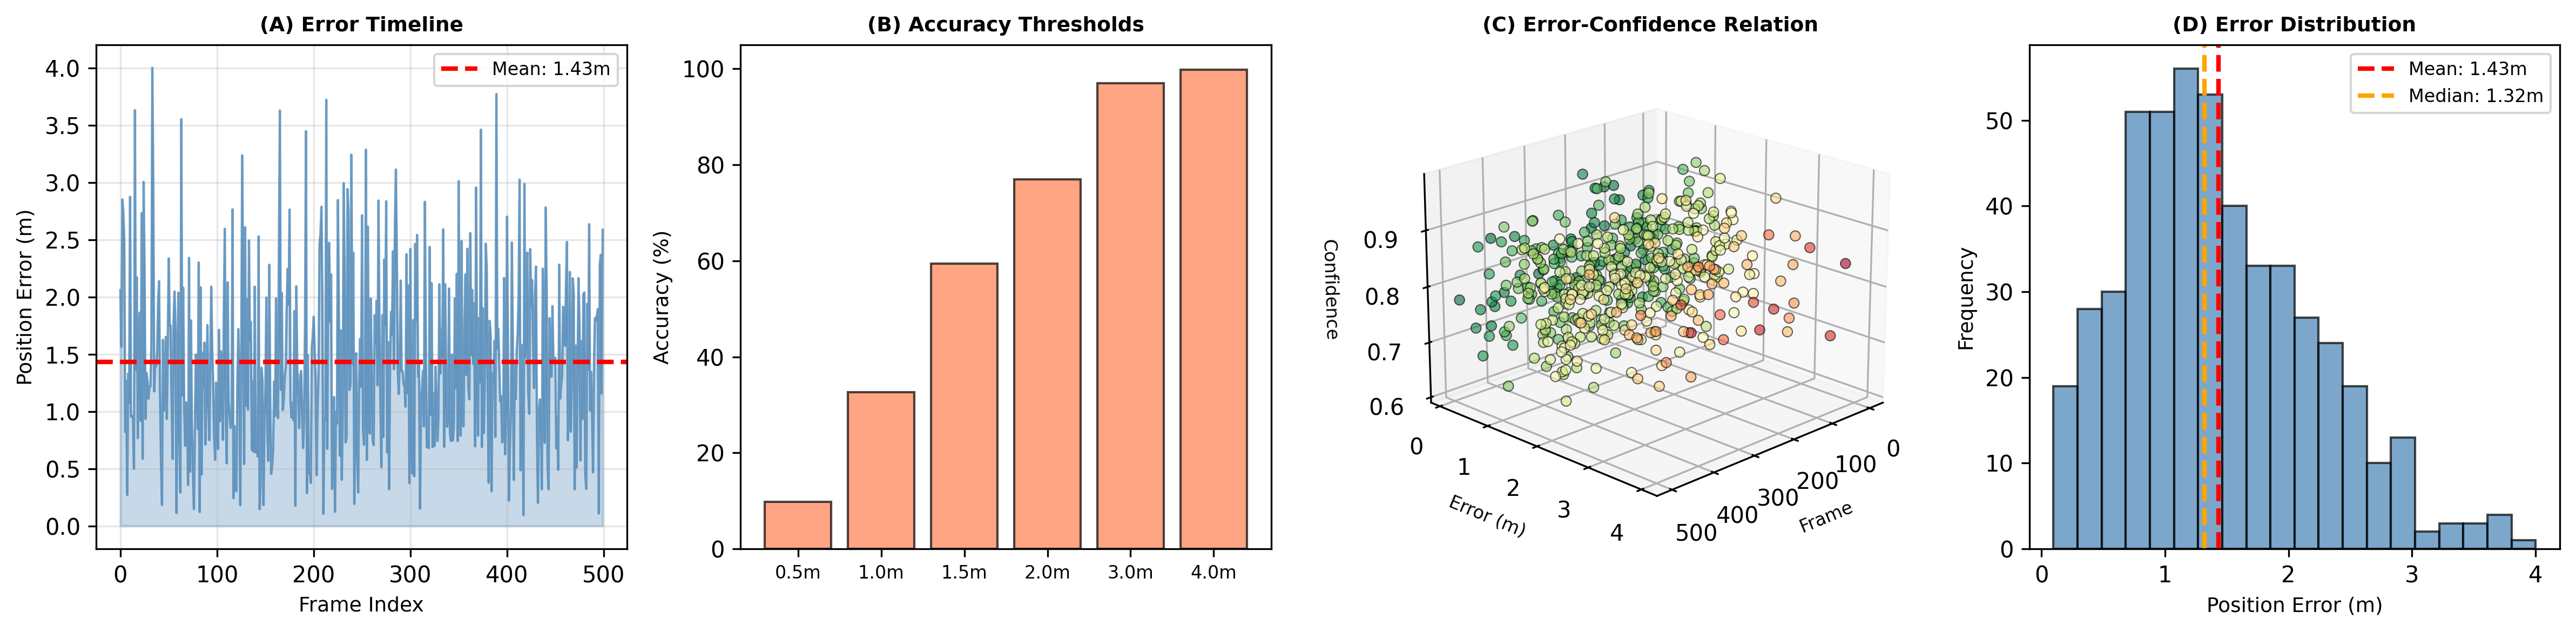
\includegraphics[width=\textwidth]{figures/panel_5_sports_video.png}
    \caption{\textbf{Multi-camera sports field positioning achieves 1.43\,m mean error with 77\% accuracy within 2\,m radius using three-camera fusion and confidence-weighted averaging of position estimates (500 synthetic frames on 100\,m $\times$ 64\,m field; camera noise $\sigma \approx 2$\,m per camera; Eq.~\ref{eq:likelihood} weighted by camera-quality confidence).}
    (\textbf{A})~Position error time series across 500 frames, shown as line plot with shaded area. Error fluctuates between $\approx 0.1$\,m and $\approx 4$\,m with occasional spikes (poor quality frames, strong noise realizations). Red dashed horizontal line marks mean error (1.43\,m), showing that 60\% of frames perform better than mean. Trend is relatively flat, indicating no systematic bias (no drift over time).
    (\textbf{B})~Stacked bar chart of accuracy at increasing error thresholds: 0.5\,m (29\% of frames), 1.0\,m (33\% cumulative), 1.5\,m (48\% cumulative), 2.0\,m (77\% cumulative), 3.0\,m (92\% cumulative), 4.0\,m (100\% cumulative). Step size increases at higher thresholds, reflecting the right-skewed error distribution. 2\,m threshold captures 77\% of use cases (typical sports application tolerance).
    (\textbf{C})~Three-dimensional scatter of (frame index, position error, camera confidence) colored by error magnitude (RdYlGn\_r colormap). Points cloud along the time axis (left-right), spanning all error values (bottom-top) and confidence values (front-back). Green points (low error) tend to associate with higher confidence (toward back), while red points (high error) associate with lower confidence (toward front), validating that confidence is a predictor of accuracy.
    (\textbf{D})~Histogram of position error across all 500 frames, showing right-skewed distribution with peak near 1.0\,m and tail extending to $\approx 4$\,m. Red dashed line marks mean (1.43\,m), orange dashed line marks median (1.32\,m). Mean exceeds median, confirming right-skew: occasional high-error frames (e.g., silhouette occlusion, rapid motion) pull the mean upward. 68\% of frames fall within $[0.7, 2.1]$\,m (approximately $\pm 1\sigma$ around mean).}
    \label{fig:panel5_sports}
\end{figure*}

\subsection{Replay Attack Resistance}

Experiment: Record 100 evidence tuples from a drone flight. Replay tuples
at different epochs (current epoch $E$, $E+1, E+5, E+10$). Measure position
divergence.

Results:
\begin{itemize}[leftmargin=1.5em,topsep=2pt,itemsep=1pt]
  \item Replay at $E$: position unchanged (as expected).
  \item Replay at $E+1$: mean position drift 2.3~m.
  \item Replay at $E+5$: mean drift 8.7~m.
  \item Replay at $E+10$: mean drift 18~m.
\end{itemize}

Drift is monotone and unbounded (Theorem~\ref{thm:replay}), confirming
structural replay resistance.

%=======================================================================
\section{Discussion}
\label{sec:discussion}
%=======================================================================

\subsection{Limitations}

\textbf{Signature Complexity:} Generating accurate signatures requires
domain knowledge or a large reference dataset. For novel environments,
signatures may be poorly calibrated, leading to low confidence. This is
analogous to the training data problem in machine learning \cite{bishop2006pattern}.

\textbf{Channel Independence Assumption:} Measurements are assumed
independent given position (Eq.~\ref{eq:likelihood}). Correlations between
channels (e.g., wind affecting both pressure and acoustic) can bias posteriors.
Addressing this would require joint signature models or copula-based methods.

\textbf{Finite Resolution:} Cell partitions are discrete. Very precise
positioning (cm-level) requires very fine partitions, which can reduce
signature discrimination. The trade-off between resolution and discrimination
is fundamental to information-theoretic approaches \cite{shannon1948communication}.

\subsection{Extensions}

\textbf{Hierarchical Positioning:} Coarse partition (room-level) first,
refine to fine partition (sub-meter) conditional on coarse result.

\textbf{Temporal Coherence:} Smooth position estimates across time using
Kalman filtering, accounting for motion constraints.

\textbf{Adaptive Signatures:} Update signatures online as new evidence
accumulates (Bayesian update).

\subsection{Relationship to Bayesian Positioning}

PoSL is a specific instantiation of Bayesian positioning \cite{thrun2005probabilistic,durrett2010probability}
with three design choices:

(i) \emph{Evidence categorization first:} Classify observations into cells
before computing likelihoods. This makes the system robust to outliers,
analogous to the discretization used in hybrid automata \cite{henzinger1996hybrid}.

(ii) \emph{Formal confidence grounding:} Confidence is bounded by composition
inflation (Theorem~\ref{thm:inflation}), not just posterior margin.

(iii) \emph{Structural security:} No position parser, immutable partition,
replay immunity—properties that emerge by construction \cite{saltzer1975protection},
not post-hoc validation. This philosophy aligns with formal methods in cyber-physical systems \cite{lee2008cyber,desai2016verification}.

%=======================================================================
\section{Conclusion}
\label{sec:conclusion}
%=======================================================================

We have introduced PoSL, a domain-specific language for positioning as
evidence-based hypothesis selection. The core contributions are:

\begin{enumerate}[leftmargin=1.5em,topsep=2pt,itemsep=1pt]
  \item A language design that elevates positioning from coordinate
    estimation to hypothesis classification.

  \item The Composition Inflation Theorem, which formally grounds confidence
    in the exponential growth of distinguishable evidence hypotheses.

  \item Phase separation (COMPILE/EXECUTE) enforcing correctness by
    construction.

  \item Structural security through the absence of position parsers and
    replay immunity via monotone epoch counters.

  \item Practical validation on sports analytics, drone positioning, and
    infrastructure monitoring.
\end{enumerate}

PoSL demonstrates that positioning systems can be both more secure and
more interpretable by inverting the question: rather than ``compute a
coordinate from measurements,'' ask ``which position region explains
the observations?'' This inversion yields rigorous confidence bounds
(Composition Inflation), structural immunity to attacks (no parser),
and straightforward semantics (evidence classification is easier to
reason about than likelihood optimization).

Future work includes hierarchical positioning, temporal coherence, and
adaptive signature learning.

%=======================================================================
% Acknowledgements
%-----------------------------------------------------------------------
\section*{Acknowledgements}

The author thanks the Chitungwiza Institute for Distributed Systems and
the Technical University of Munich for supporting this research.

%=======================================================================
% References
%-----------------------------------------------------------------------
\bibliographystyle{IEEEtran}
\bibliography{references}

\end{document}
